\documentclass{article}
\usepackage[T1]{fontenc}
\usepackage{lmodern}
\usepackage{graphicx}
\usepackage{amsmath,amssymb}
\usepackage[a4paper,margin=2cm]{geometry}
\usepackage[absolute,overlay]{textpos}
\setlength{\TPHorizModule}{1mm}
\setlength{\TPVertModule}{1mm}
\usepackage[indonesian]{babel}
\usepackage{hyperref}
\setlength{\emergencystretch}{2em}
% unit: Halaman 10

\begin{document}

% === Halaman 10 (python/native) ===

10

DEKRIPSI:

Cipherteks: 

WHPXL VDBD GL MHPEDWDQ PHUDK QDQWL PDODP

•

c1 = ‘W’ = 22 → p1 = D(22) = (22 – 3) mod 26 = 19 = ‘t’

•

c2 = ‘H’ = 7 → p2 = D(7) = (7 – 3) mod 26 = 4 = ‘e’

•

c3 = ‘P’ = 15 → p3 = D(15) = (15 – 3) mod 26 = 12 = ‘m’

•

c4 = ‘X’ = 23 → p4 = D(23) = (23 – 3) mod 26 = 20 = ‘u’    

•

 c5 = ‘L’ = 11 → p5 = D(11) = (11 – 3) mod 26 = 8 = ‘i’

•

…dst


Plainteks: temui saya di jembatan merah nanti malam

% deskripsi: gambar native xref 66
\noindent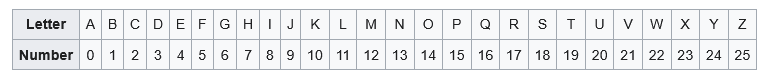
\includegraphics[width=0.85\textwidth]{../../images/python/page_010_img_01.png}

\end{document}
